\documentclass{beamer}
\usetheme{Boadilla}

\title{Automatic polishing machine}
\subtitle{TRITIUM}
\author{Marcos Martínez Roig}
\institute{University of Valencia}
\date{\today}

\begin{document}

\begin{frame}
\titlepage
\end{frame}

\begin{frame}
\frametitle{Outline}
\tableofcontents
\end{frame}

\section{First day}
\section{Second day}
\section{Third day}
\section{fourth day}
\section{fifth day}


\begin{frame}
\frametitle{First day (in the morning)}
Building of the machine and soldering of the wires:
\begin{figure}[hbtp]
\centering
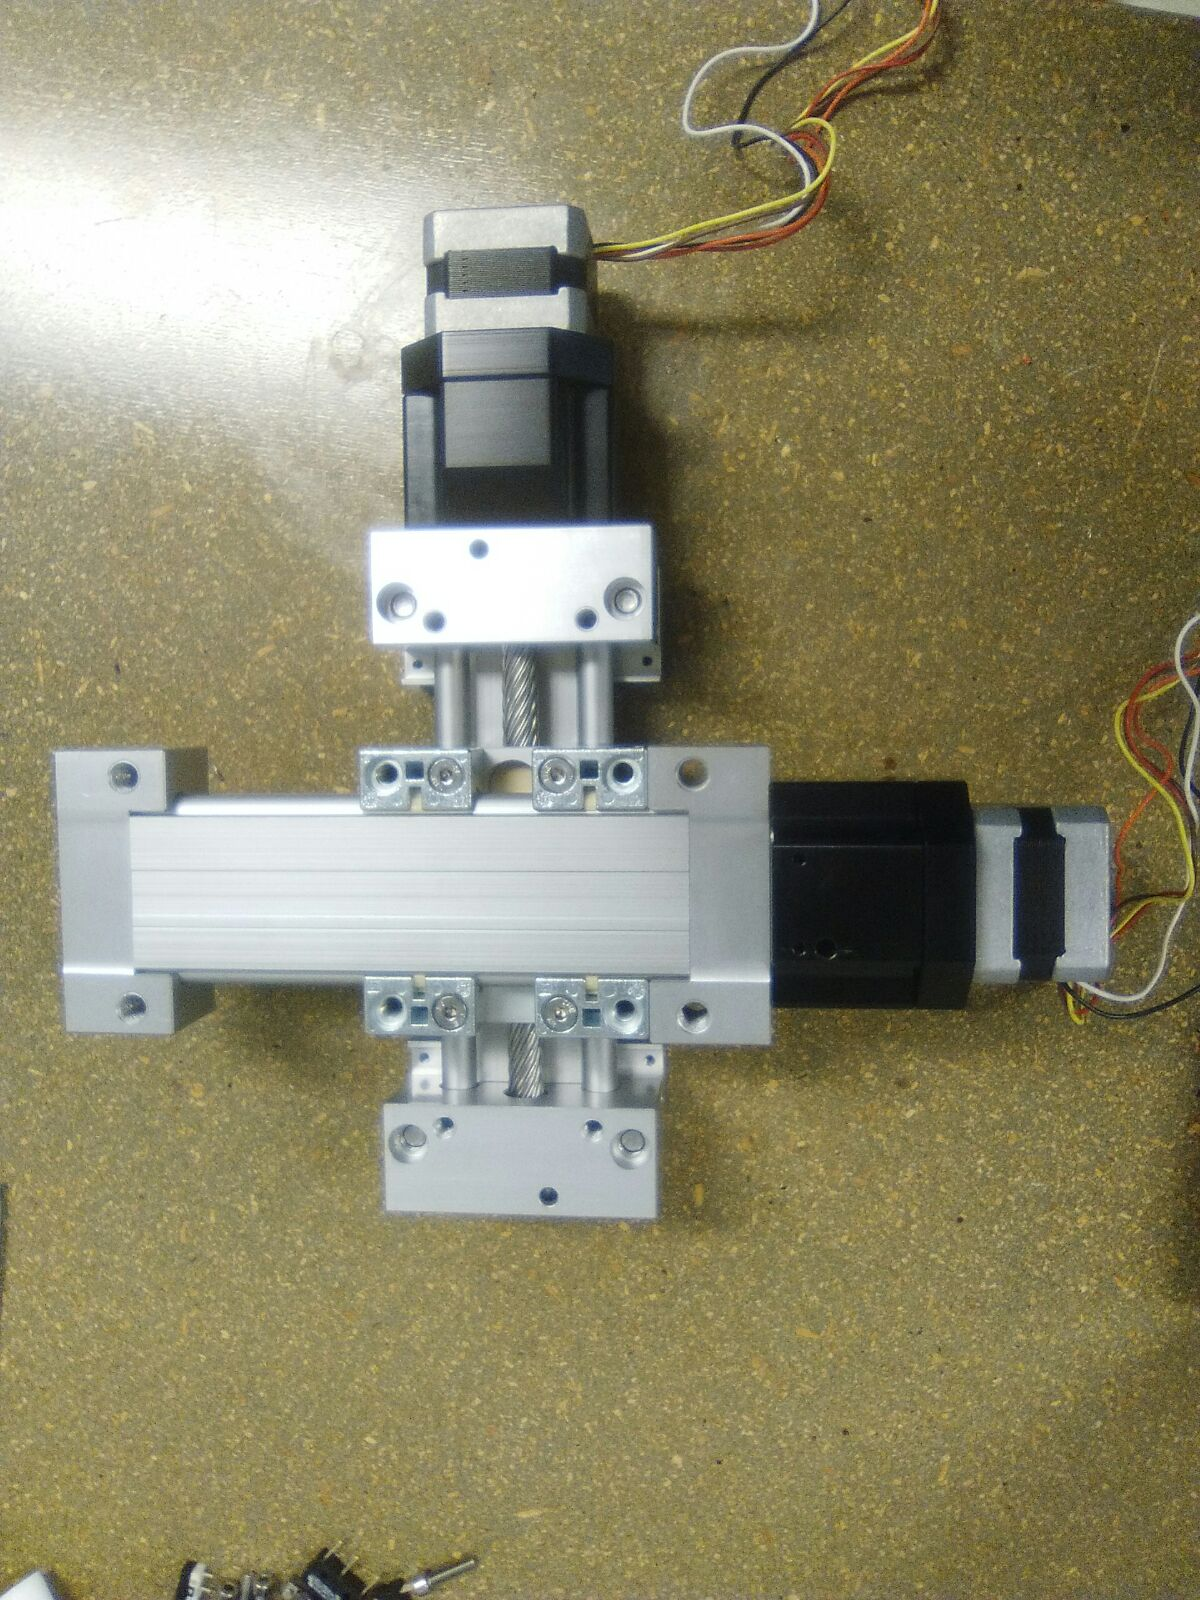
\includegraphics[scale=0.1]{Picture1.jpeg}
\caption{Machine}
\end{figure}
\end{frame}


\begin{frame}
\frametitle{First day (in the morning)}
Building of the machine and soldering of the wires:

\begin{columns}
\column{0.5\textwidth}

\begin{figure}[hbtp]
\centering
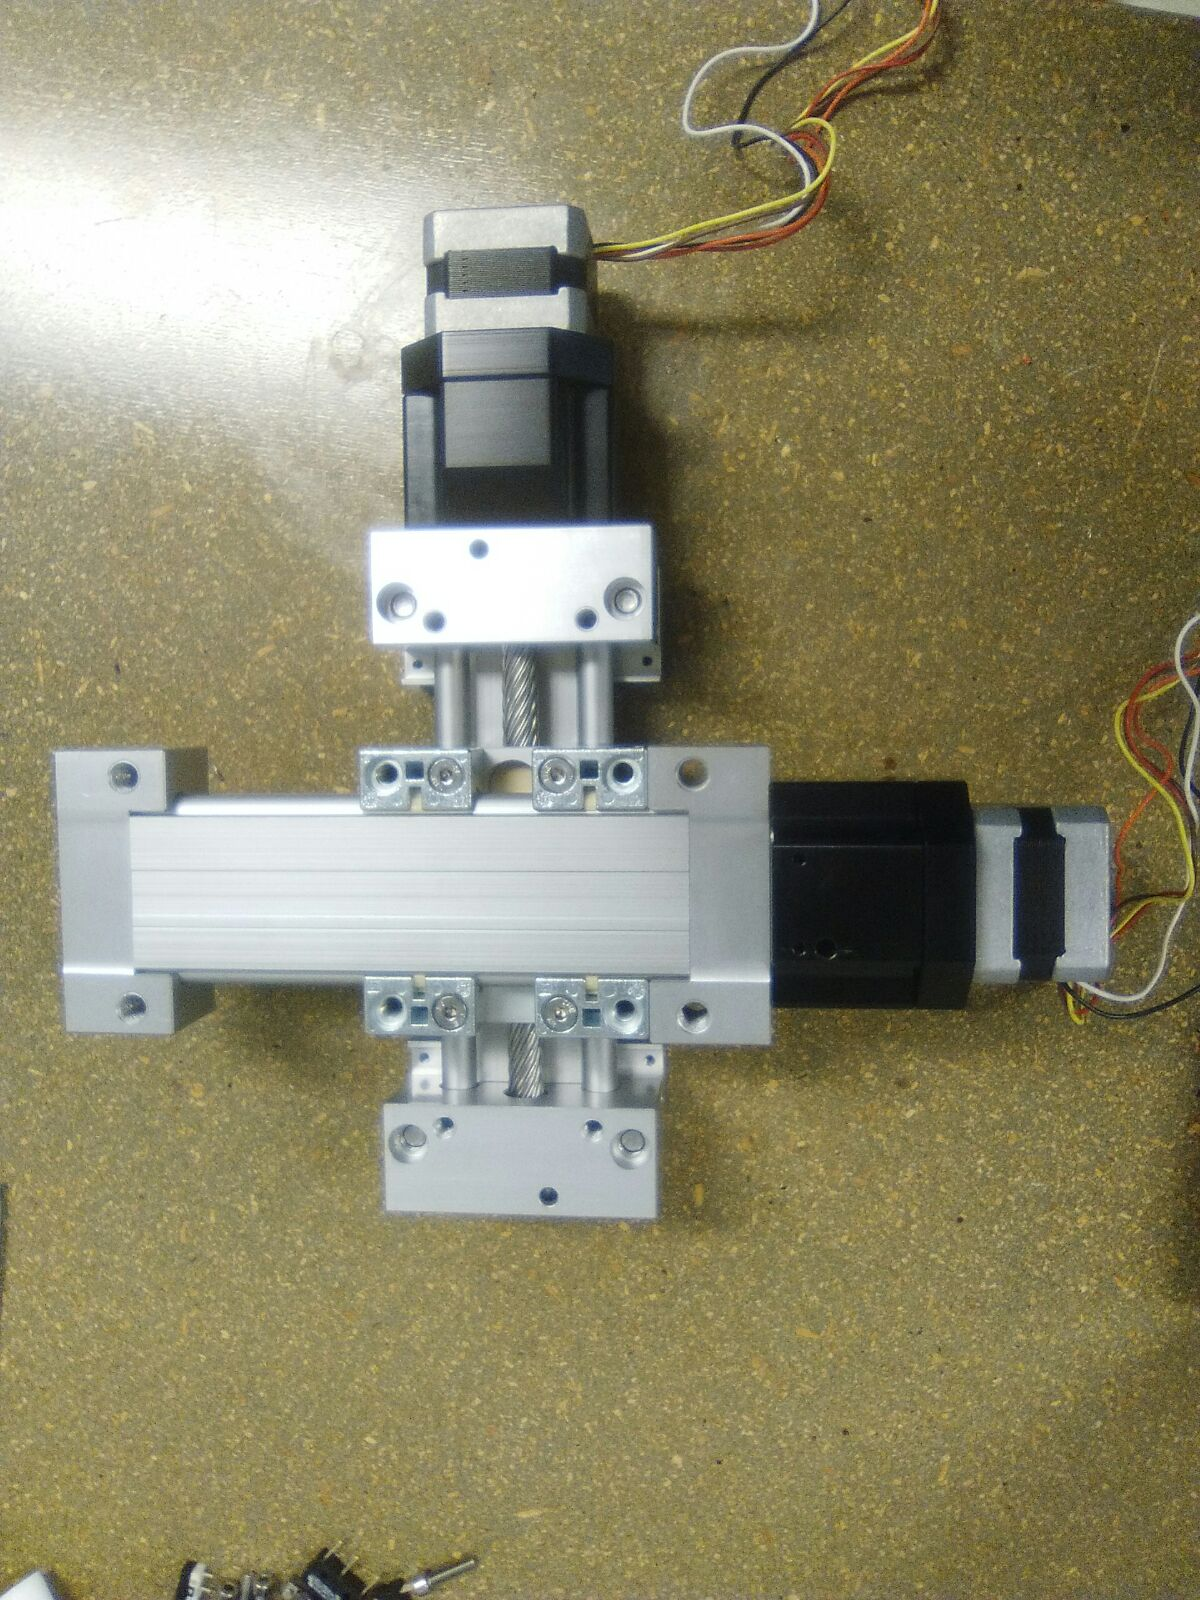
\includegraphics[scale=0.1]{Picture1.jpeg}
\caption{Machine}
\end{figure}

\column{0.5\textwidth}

We checked this one (It work good).

\begin{alertblock}{Problem}
\begin{itemize}
\item{}The speed of this machine is too slow
\item{}End of the way
\item{}If we use a higher speed the moviment is not soft enough
\end{itemize}

\end{alertblock}

\begin{block}{Solutions}
\begin{itemize}
\item{}Change of the motors
\item{}Using switch
\item{}For solving this problem we use a steppers
\end{itemize}
\end{block}


\end{columns}
\end{frame}





\begin{frame}
\frametitle{First day (in the morning)}
Steppers:
\begin{columns}
\column{0.5\textwidth}

\begin{figure}[hbtp]
\centering
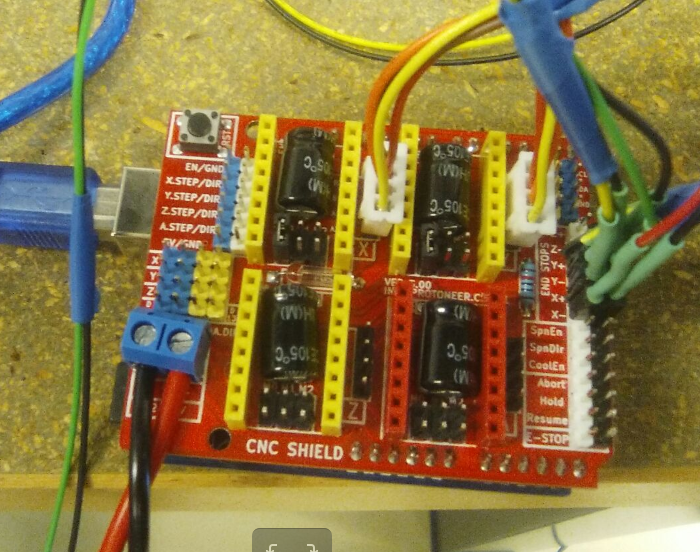
\includegraphics[scale=0.2]{Tarjeta_CNC.png}
\caption{CNC Shield}
\end{figure}

\column{0.5\textwidth}

\begin{figure}[hbtp]
\centering
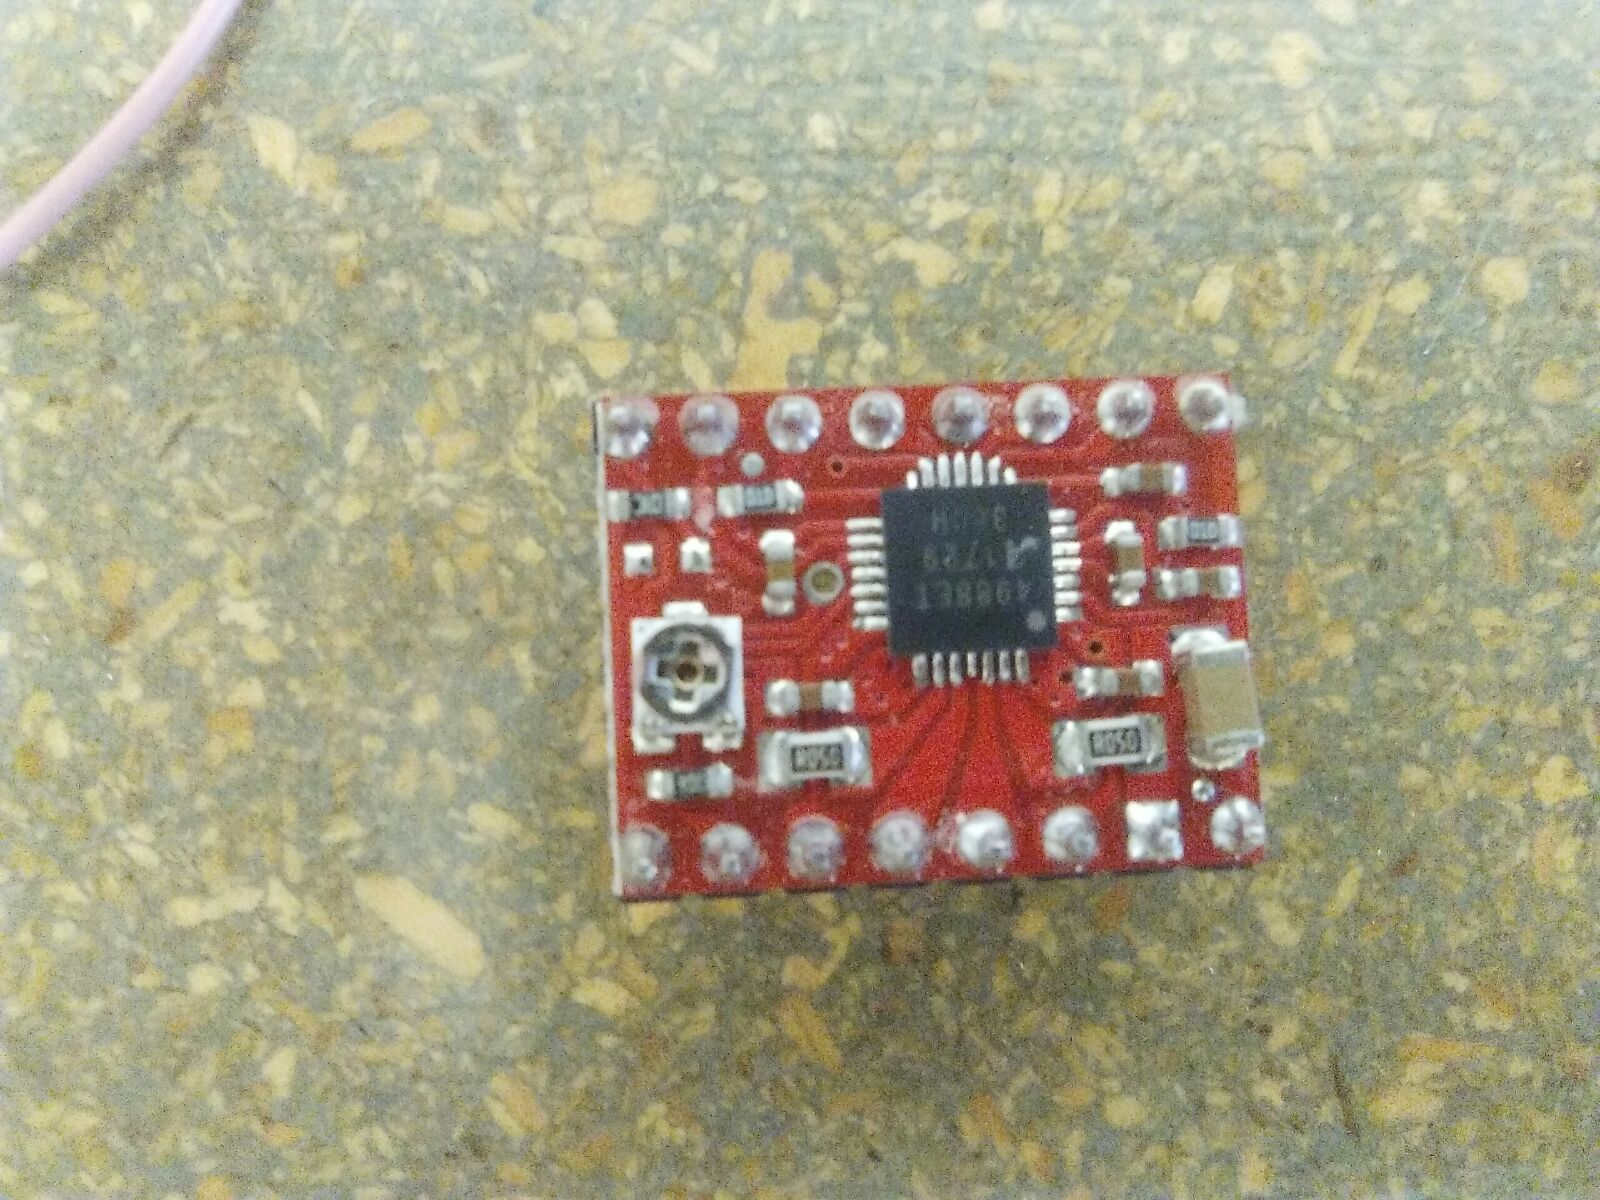
\includegraphics[scale=0.1]{Driver.jpeg}
\caption{Driver (A4988)}
\end{figure}

\end{columns}
\end{frame}

\begin{frame}
\frametitle{First day (in the morning)}
Steppers:
\begin{columns}
\column{0.5\textwidth}

\begin{figure}[hbtp]
\centering
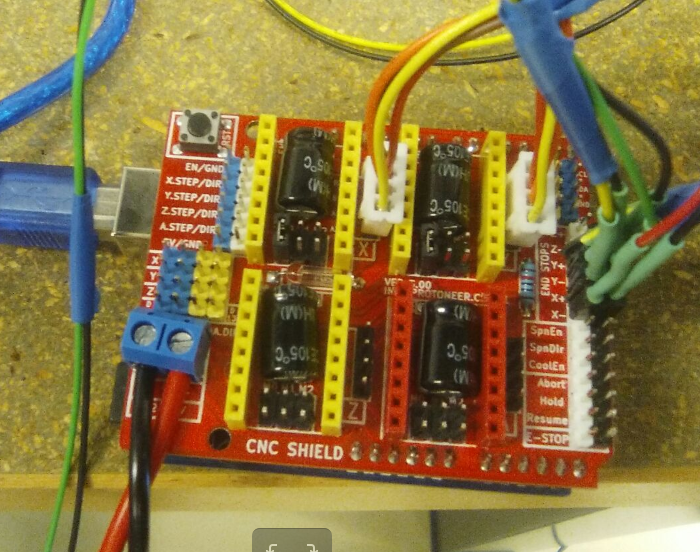
\includegraphics[scale=0.2]{Tarjeta_CNC.png}
\caption{CNC Shield}
\end{figure}

\column{0.5\textwidth}

\begin{figure}[hbtp]
\centering
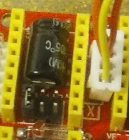
\includegraphics[scale=0.5]{Stepper.png}
\caption{Module}
\end{figure}

\end{columns}
\end{frame}

\begin{frame}
\frametitle{First day (in the morning)}
Steppers:
\begin{columns}
\column{0.5\textwidth}

\begin{figure}[hbtp]
\centering
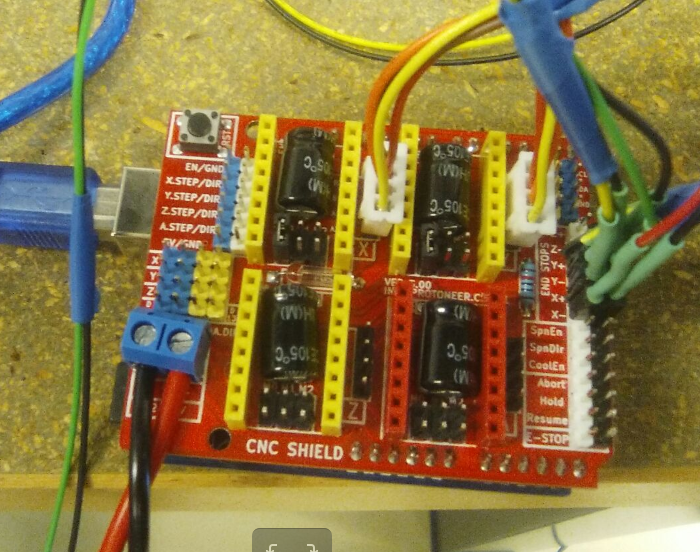
\includegraphics[scale=0.2]{Tarjeta_CNC.png}
\caption{CNC Shield}
\end{figure}

\column{0.5\textwidth}

\begin{figure}[hbtp]
\centering
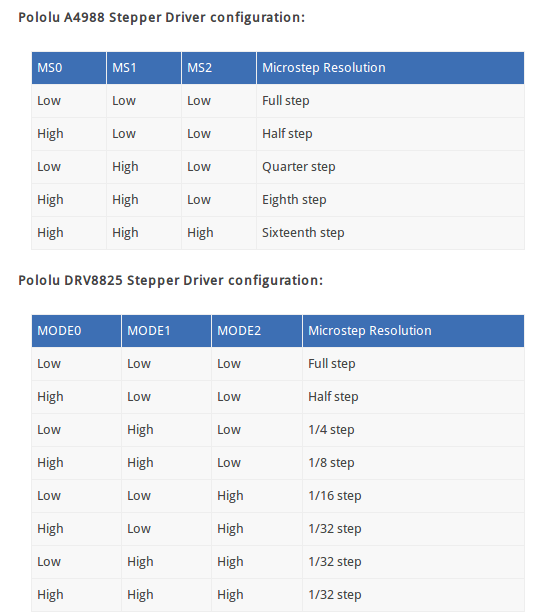
\includegraphics[scale=0.3]{Especificaciones_Steppers.png}
\caption{Configuration steppers}
\end{figure}

\end{columns}
\end{frame}

\begin{frame}
\frametitle{First day (in the afternoon)}
Building of the special pieces for holding the switch with a 3D printer:

\begin{columns}
\column{0.5\textwidth}

\begin{figure}[hbtp]
\centering
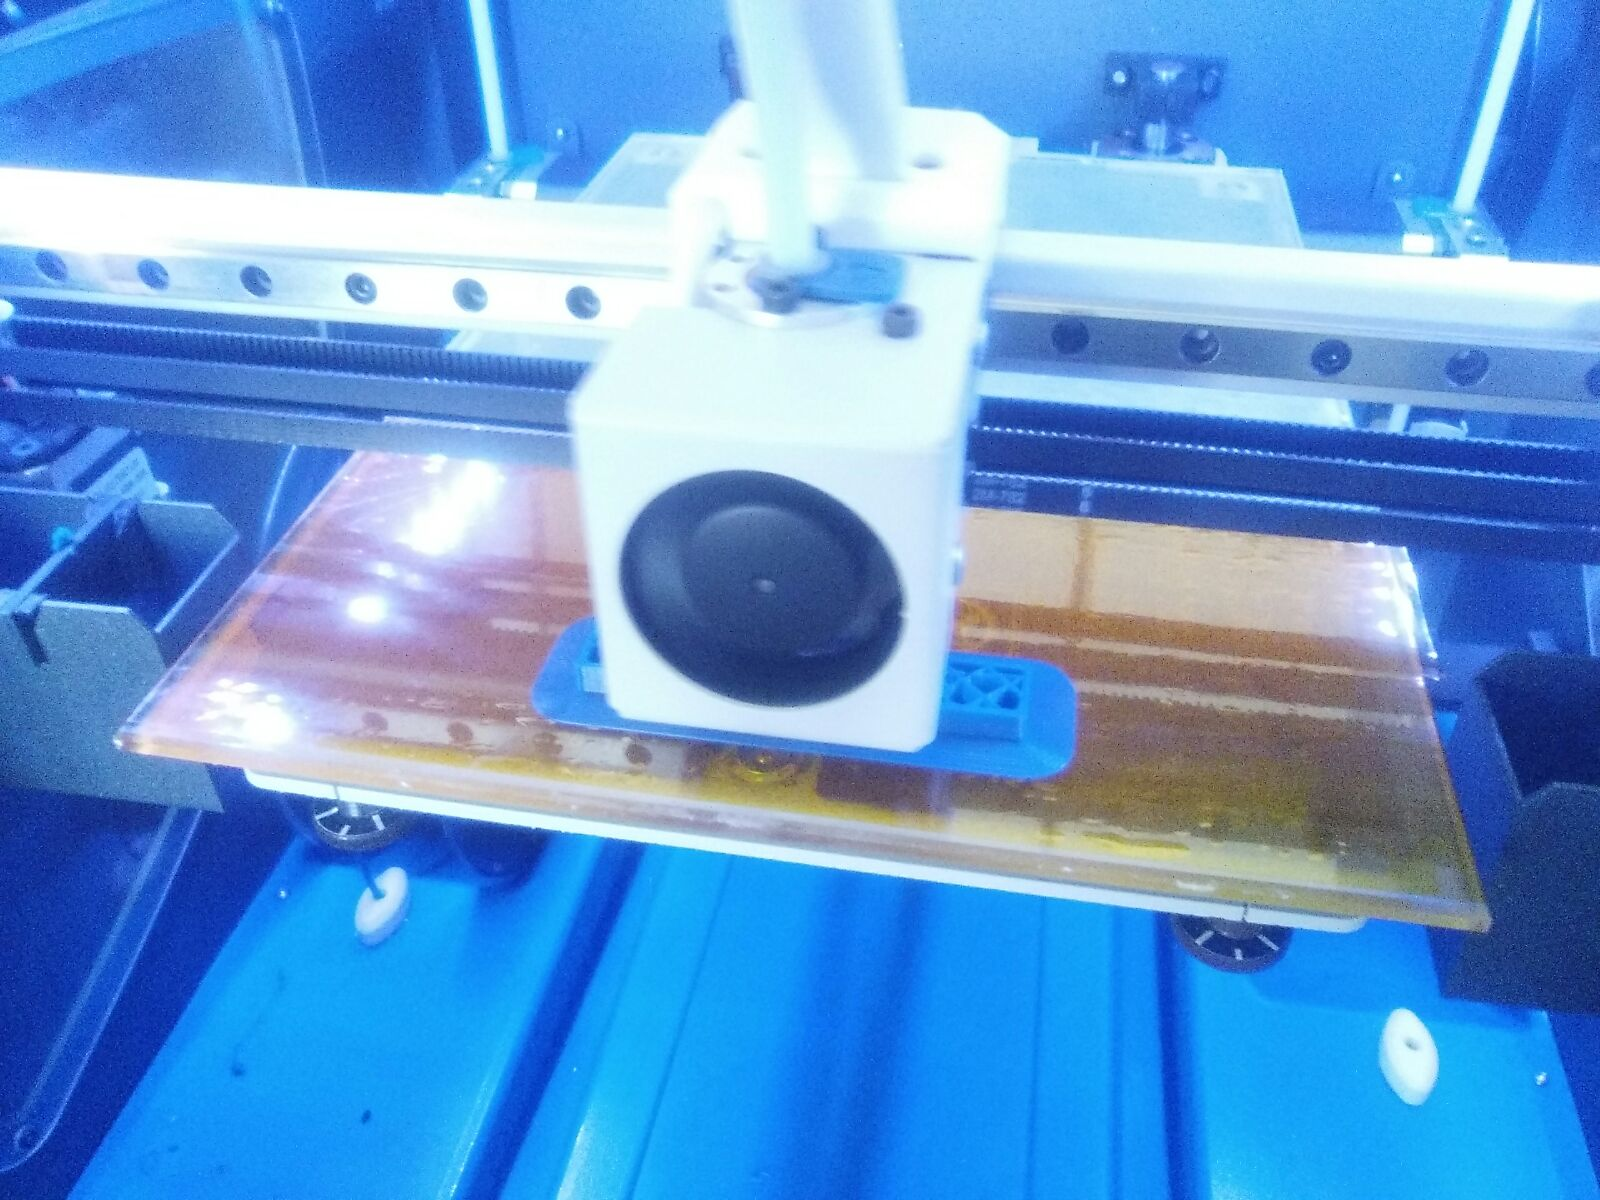
\includegraphics[scale=0.1]{3Dprinter.jpeg}
\caption{Process of the building of this pieces}
\end{figure}

\column{0.5\textwidth}

\begin{figure}[hbtp]
\centering
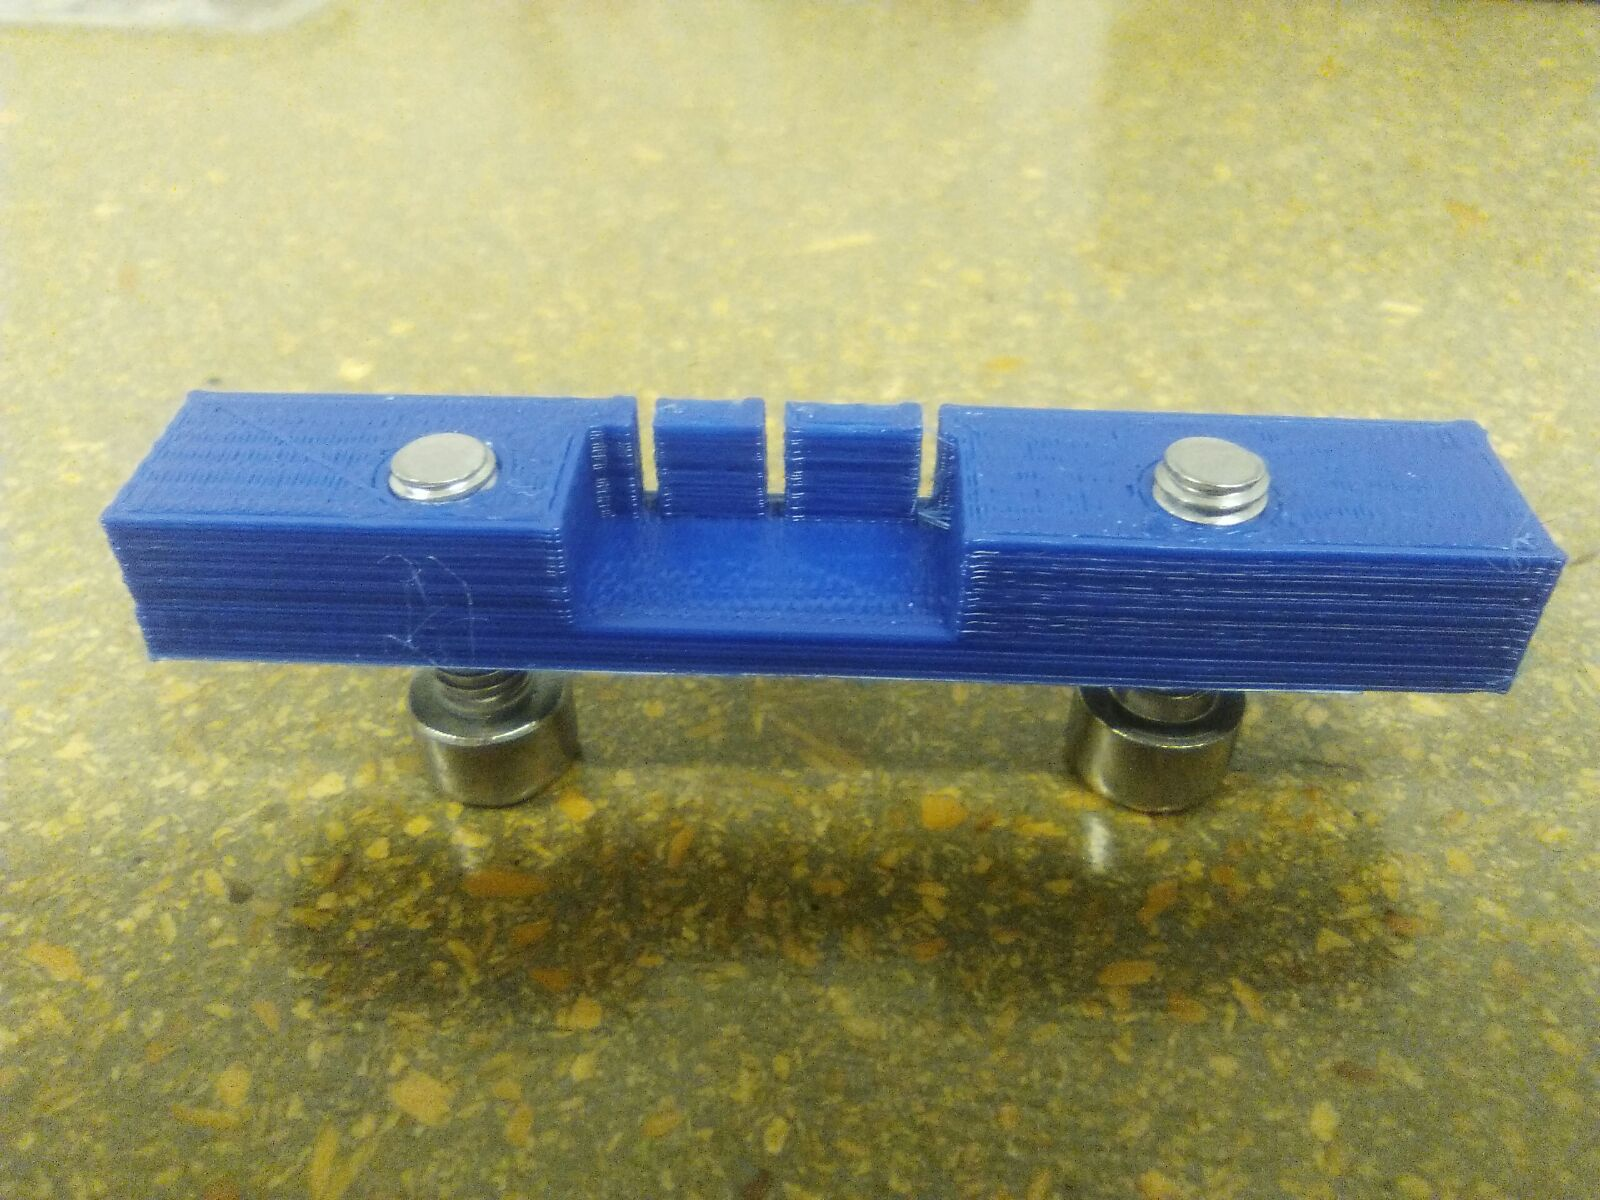
\includegraphics[scale=0.1]{Switch_piece.jpeg}
\caption{Piece for holding a switch}
\end{figure}

\end{columns}

We had some problems with this 3D printer and we lost that afternoon
\end{frame}

\begin{frame}
\frametitle{Second day (in the morning)}
How it works?
\begin{columns}
\column{0.5\textwidth}

\begin{figure}[hbtp]
\centering
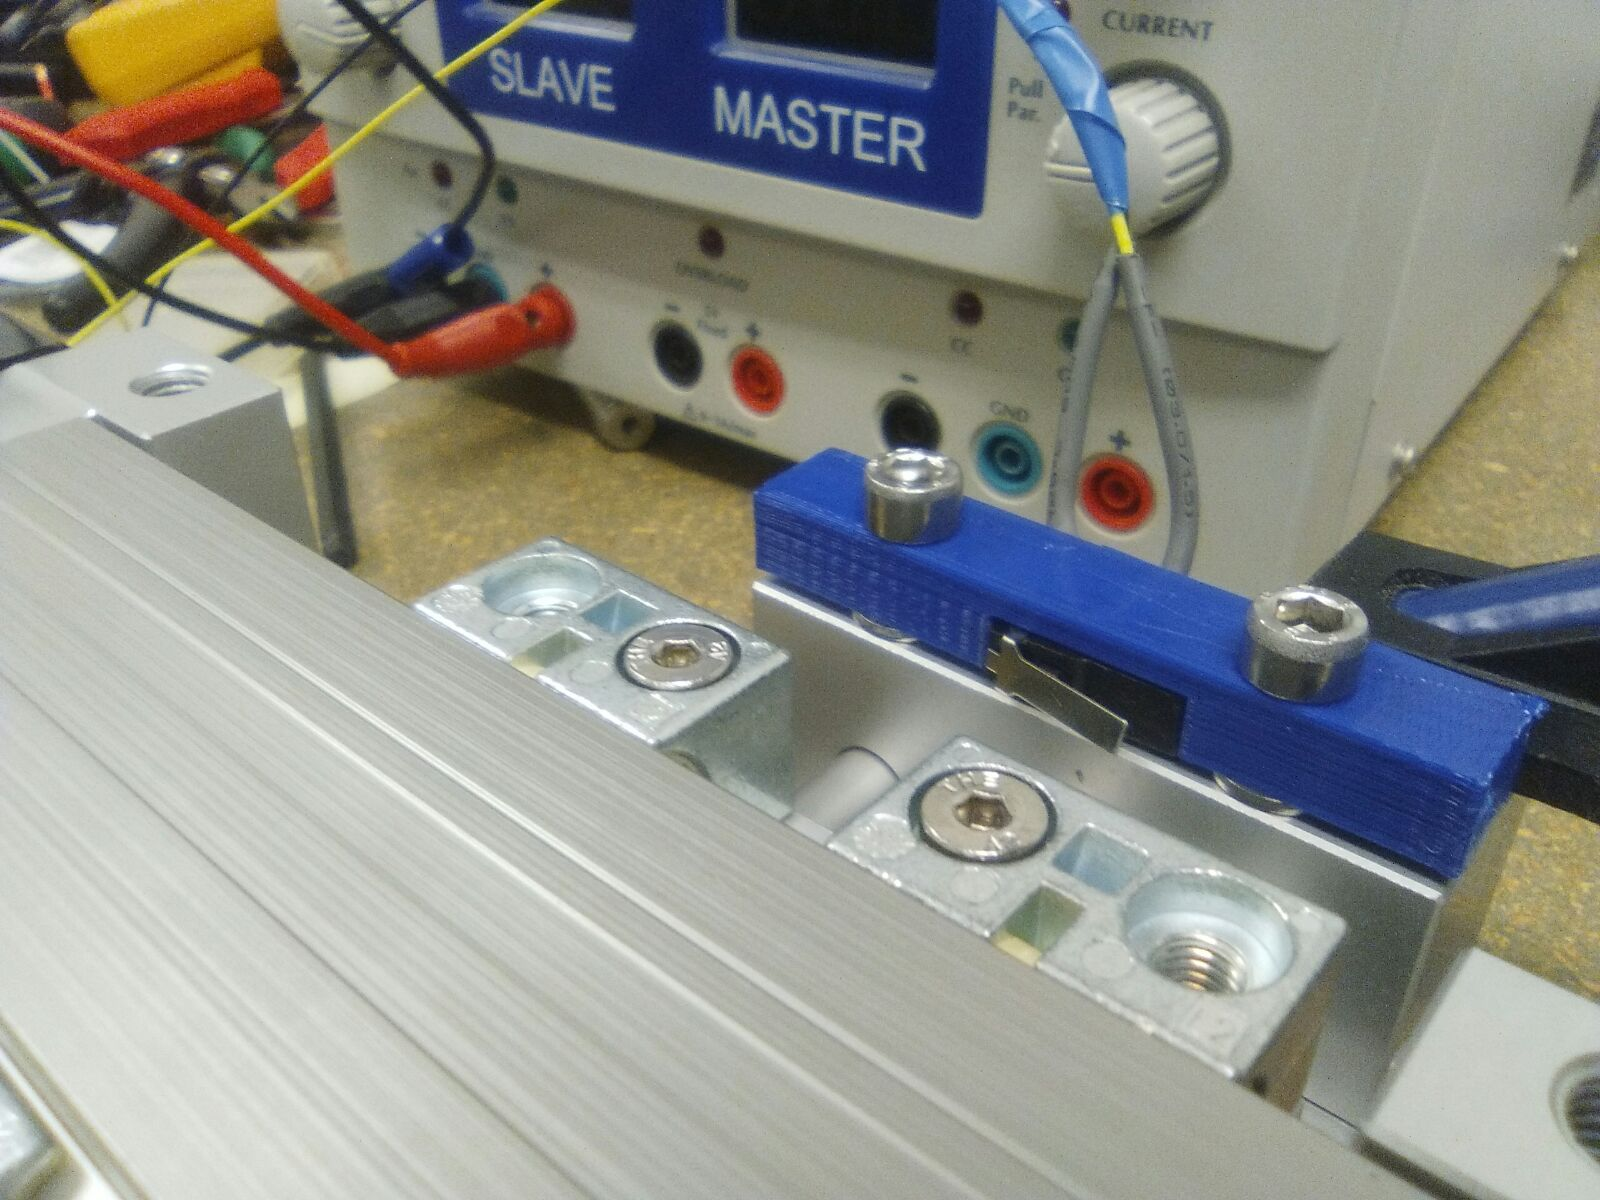
\includegraphics[scale=0.1]{swithc_piece_set_up.jpeg}
\caption{Piece for holding a switch in the moachine}
\end{figure}

\column{0.5\textwidth}

\begin{figure}[hbtp]
\centering
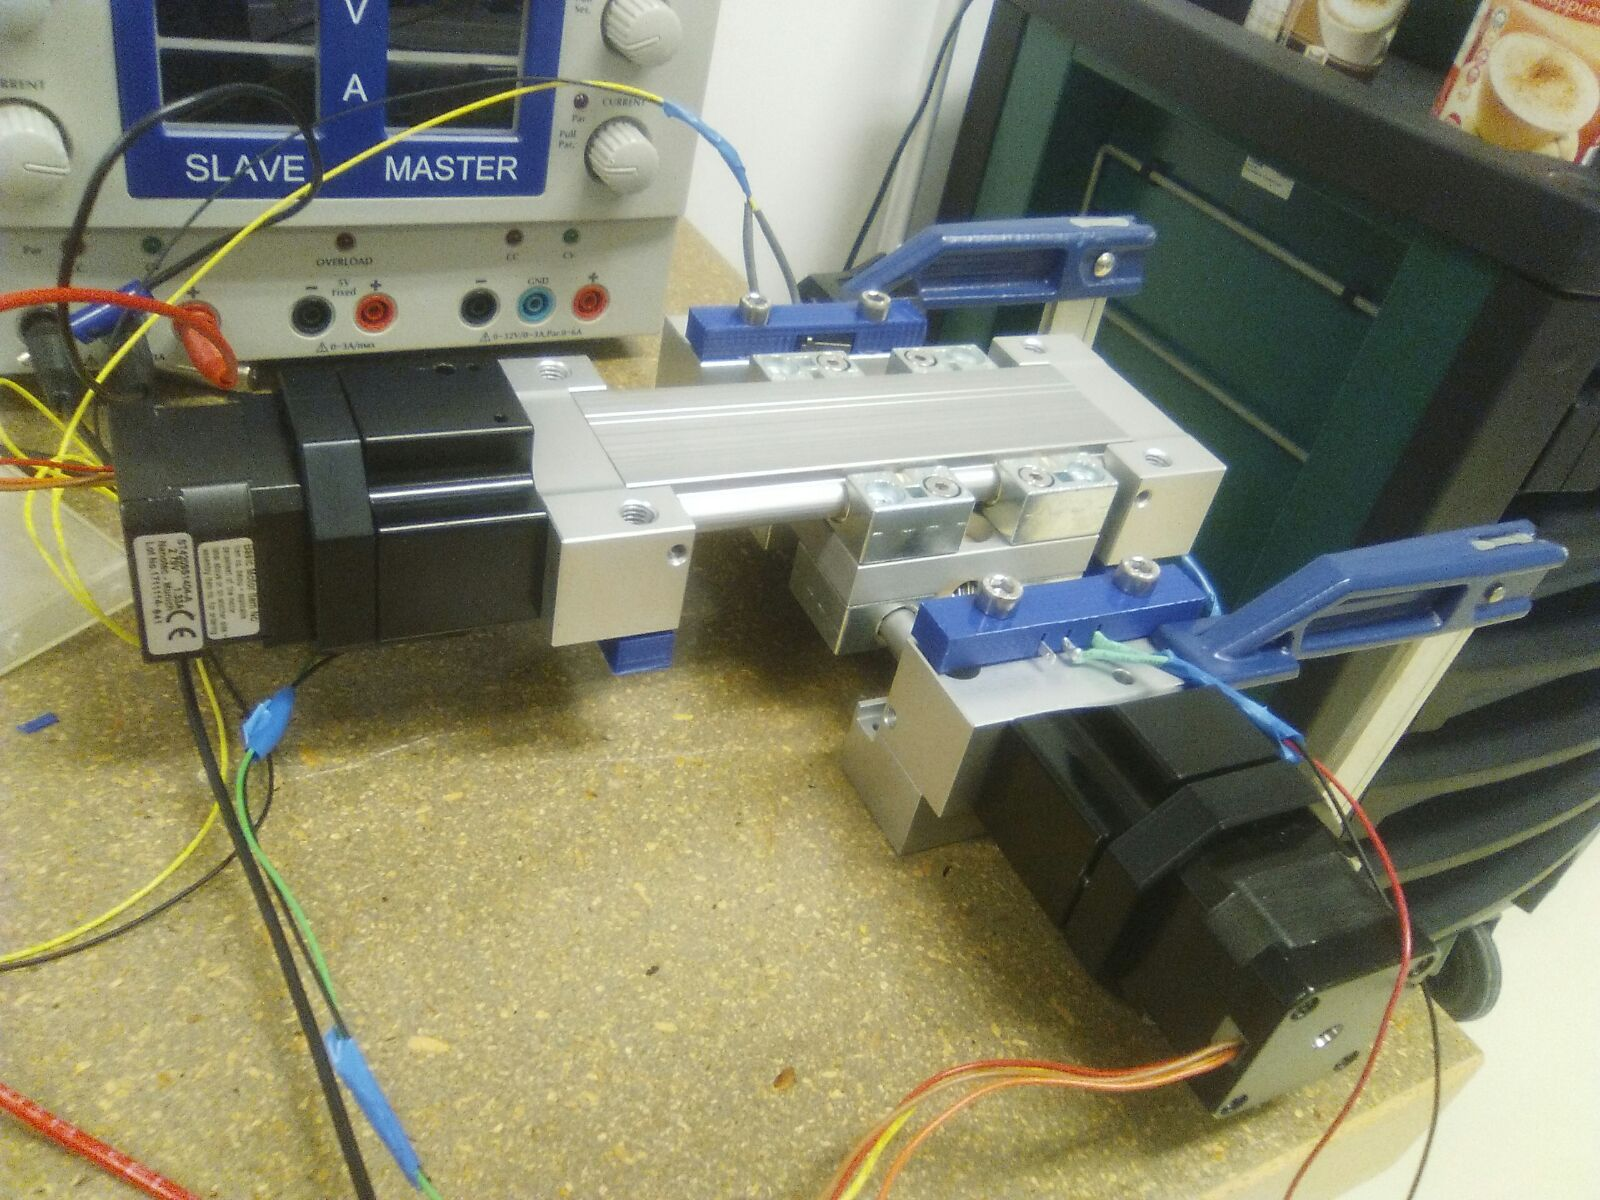
\includegraphics[scale=0.1]{swithc_pieces_set_up.jpeg}
\caption{Piece for holding a switch in the moachine}
\end{figure}

\end{columns}
\end{frame}


\begin{frame}
\frametitle{Second day (in the afternoon)}
\begin{itemize}
\item{} Now we have got that this machine work softly and with hard limits.
\item{} The problem just now is that, when we try to use a higher speed, these motors lose some steps.
\begin{itemize}
\item{} Problem with the motors. 
\end{itemize}


\begin{columns}
\column{0.5\textwidth}

\begin{figure}[hbtp]
\centering
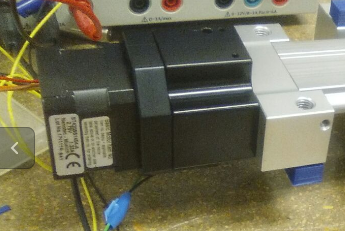
\includegraphics[scale=0.5]{motor_good.png}
\caption{Motor with which this device work good}
\end{figure}

\column{0.5\textwidth}

\begin{figure}[hbtp]
\centering
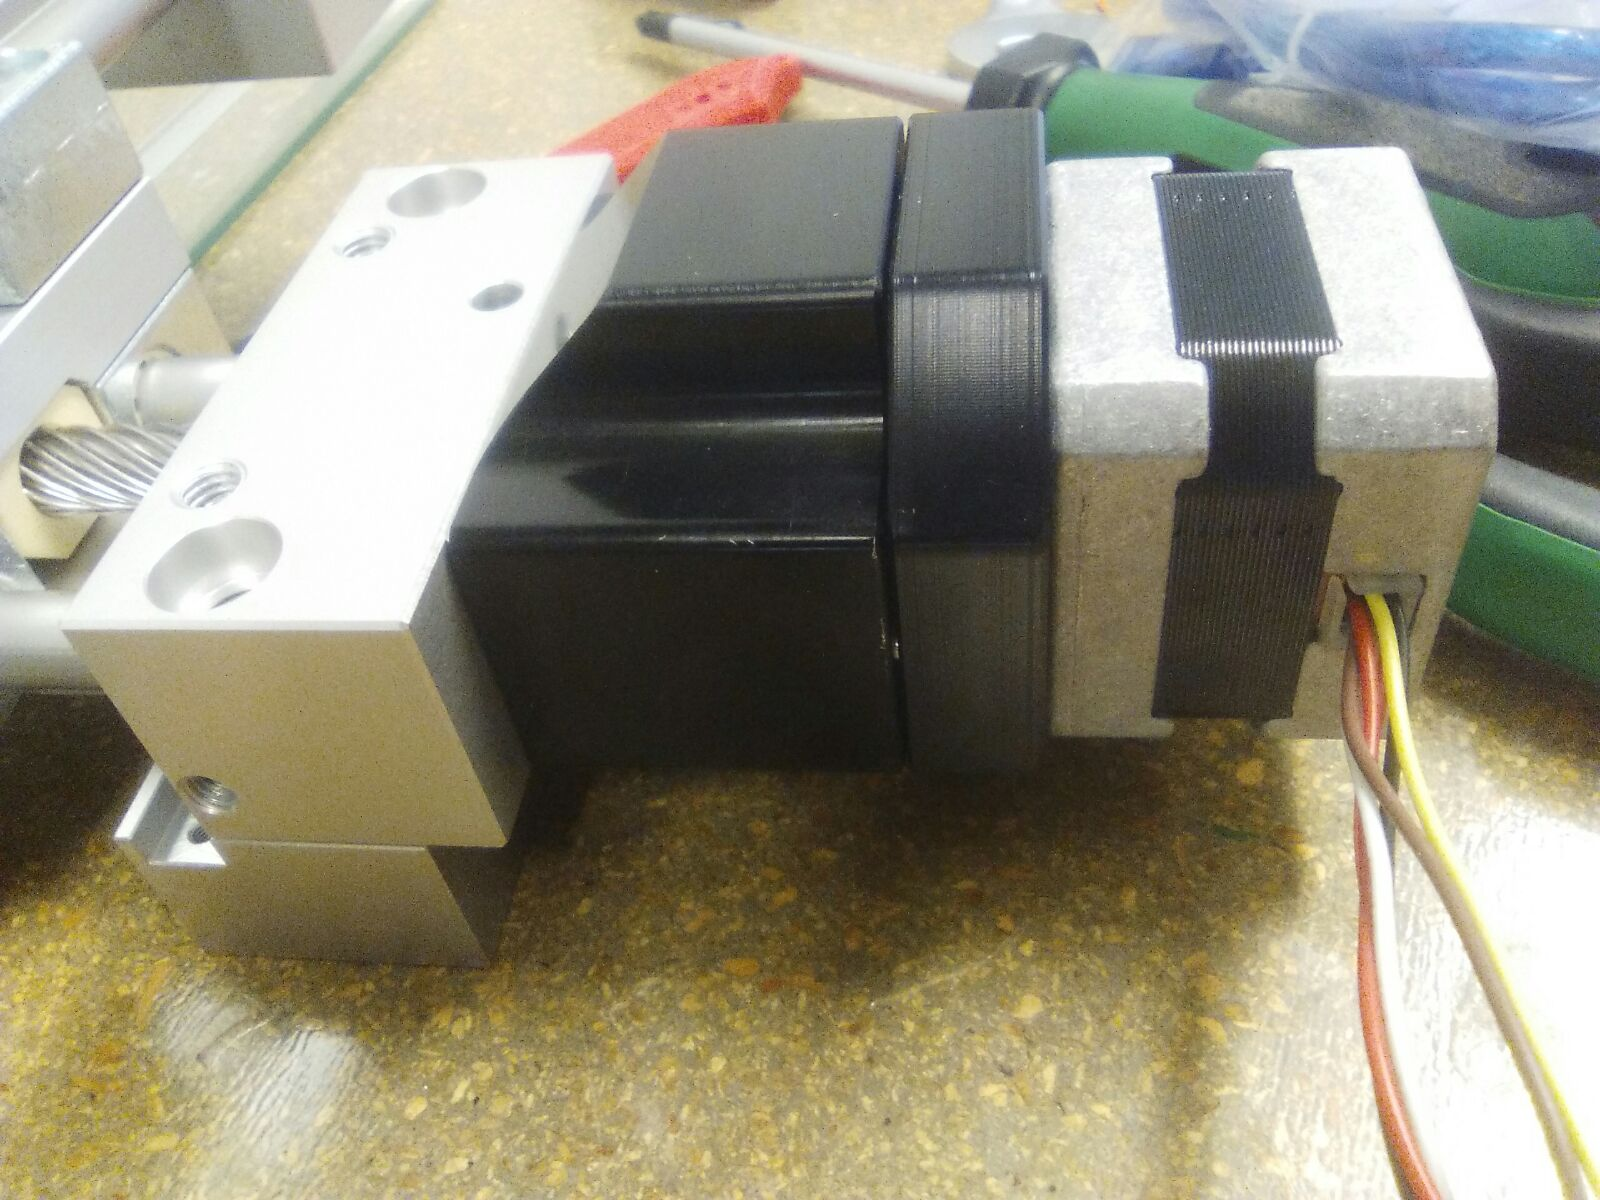
\includegraphics[scale=0.1]{motor_bad.jpeg}
\caption{Motor with which this device work bad}
\end{figure}

\end{columns}

\item{} We have lose some time with this problem.
\end{itemize}
\end{frame}


\begin{frame}
\frametitle{Third day (in the morning/afternoon)}
\begin{alertblock}{We observed other problem:}
If we turn off this machine and we move this one handly when we turn on this one, that think that it is in a wrong position.
\end{alertblock}

\begin{block}{Solution}
We used the same switch as we use in the past for design a homing cycle.
\end{block}
 
\end{frame}

\begin{frame}
\frametitle{Third day (in the morning/afternoon)}
\begin{alertblock}{We observed other problem:}
We have seen that these switchs don't work. 
\end{alertblock}

\begin{block}{Solution}
We read that this machine start with the Z axis and, next, follow with the X and Y axis, both at the same time. Quick solution: Other motor with other switch.
\end{block}
 
\begin{figure}[hbtp]
\centering
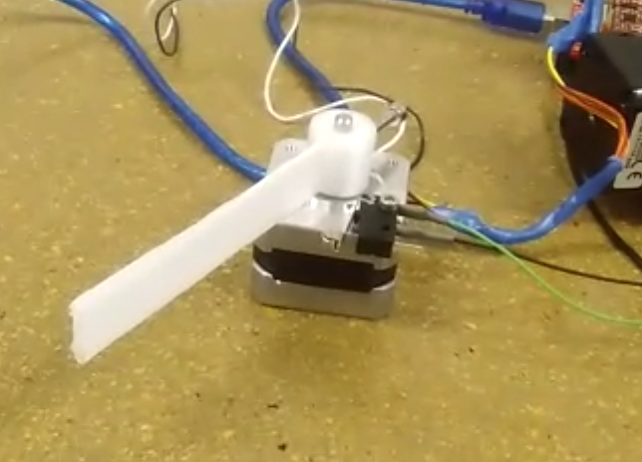
\includegraphics[scale=0.2]{Third_motor.png}
\caption{Third motor with a switch}
\end{figure} 
 
\end{frame}


\begin{frame}
\frametitle{Fourth day (in the morning/afternoon)}

\begin{alertblock}{This system don't work}
We saw that this homing cycle don't work. When we try to do this we obtained a "Alarm lock".
\end{alertblock}

\begin{block}{Solution}
We were reading a lot and we were trying some solutions like electric bridges. Finally we read that the reason of this problem is due to a confusion between several versons or GRBL. The previos versions use the pins 9,10 and 11 for this hard limits. The last version uses the pins 9, 10 and 12.
The solution was connect this Z limit in the "enable" pin, and not in the "limit Z" pin.
\end{block}

\end{frame}

\begin{frame}
\frametitle{Fifth day (in the morning)}
 
\begin{itemize}
\item{} We were looking for some G code generators for we know how we can do different circles and we develop a G code file with several sentence for doing all this stuff automatically.
\item{} Conclusions: Finally we checked that this machine is able to:
\begin{itemize}
\item {} First thing, which this machine does when you turn on this one, is the homing cycle. You can put the position which you want to the homing cycle position.
\item{} Then, this machine go to the center of your table, which will depend on your choice in the homing cycle position.
\item{} Finally we got that this machine was able to do twenty "eights" without stoped with a fast velocity (more than 1 eight/sec).
\end{itemize}
\end{itemize}
\end{frame}

\begin{frame}
\frametitle{Fifth day (in the afternoon)}
 
\begin{itemize}
\item{} We are sure that we can improve this velocity. For this reason we try to use a different power supply which could provide with a higher intensity.
\item{} But this power supply didn't work and due to connect and disconect the feed wires without turn off the power supply we burnt the drivers. It's not important, it only cost less than one euro but we couldn't follow with this machine.
\end{itemize}
\end{frame}

\begin{frame}
\frametitle{Next step}
  
\begin{itemize}
\item{} We are going to buy some drivers. We have to think what drivers we want to buy(more intensity more cost but isn't too much).

\item{} We are going to improve this machine. We want to include a LCD screen for including several posibilities like several movements or several number of this movements. 

\begin{figure}[hbtp]
\centering
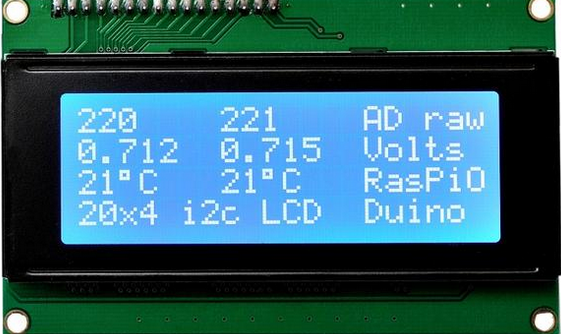
\includegraphics[scale=0.3]{Screen.png}
\caption{LCD screen}
\end{figure}
\item{} The final objective is build a independent machine
\end{itemize}


\end{frame}

\begin{frame}
\frametitle{Aveiro Tritium prototype}
  
\begin{itemize}
\item{} I cleaned their prototype and all this fibers one by one with acohol.
\item{} We did some measurements with unpolished fibers.
\begin{itemize}
\item{} We measured in several enviromentals:
\begin{itemize}
\item{} We measured in air
\item{} We measured in hiperpure water
\item{} We measured in tap water
\end{itemize}
\item{} We did this task for several conditions:
\begin{itemize}
\item{} We measured the background
\item{} We measured with iron source (We didn't see anything)
\item{} We measured with Amenicio source
\end{itemize}
\item{} Now we have to evaluate the difference between enviromentals and conditions.
\end{itemize}
\item{} Now Carlos will polish the fibers with this machine and He will repit this measures for checking all possible differences
\end{itemize}
\end{frame}



\begin{frame}
\frametitle{¿What are we going to do in august?}
\begin{itemize}

\item{} I have to develop the code for using LCD screen with arduino. Therefore I will need buy a LCD screen, whose size I have to decide yet, and some botons for manipulate the options. You can tell me some options or movements which you want that this machine have. 

\item {} We need to go on with the measurements about the veto.

\begin{itemize}
\item{} We are going to measure with several $\gamma$ source so that we can check the minimum energy which we can see with this veto (Rosa).

\item {} We will do a mapping with the source which have the best result.
\end{itemize}
\item{}  

\item{} To build the other veto which is able to detect the enviromental radiactivity.

\item{} The ADC which are installed in the laptop are working. Andres found that the threshold was different.

\item{} We have to finish the measurements about the fiber study (We can release this one)

\item{} We have to measure somethings about Tritium 1:

\begin{itemize}

\item{} 1
\item{} 2

\end{itemize}



\end{itemize}

\end{frame}

\begin{frame}
\frametitle{Beyound the meeting}

\begin{itemize}

\item{} When we will have finished this machine, I will have to replicate in order to have a machine in Valencia. It's only buy each piece and build (One day).

\item{} Do the caracterization of the SiPM. For doing this task we can replicate the work of the Marc.

\item{} We could take advantage of Carlos and reproduce the high voltage generators which he has built. He can help us.

\end{itemize}

\end{frame}




%\item{} 



\end{document}




